\documentclass[12pt, a4 paper]{article}
% Set target color model to RGB
\usepackage[inner=2.0cm,outer=2.0cm,top=2.5cm,bottom=2.5cm]{geometry}
\usepackage{setspace}
\usepackage[rgb]{xcolor}
\usepackage{environ}
\usepackage{verbatim}
\usepackage{subcaption}
\usepackage{outlines}
\usepackage{enumitem}
\usepackage{amsgen,amsmath,amstext,amsbsy,amsopn,tikz,amssymb,tkz-linknodes}
\usepackage{fancyhdr}
\usepackage{pgfplots}
\usepackage{mathtools}
\usepackage[colorlinks=true, urlcolor=blue,  linkcolor=blue, citecolor=blue]{hyperref}
\usepackage[colorinlistoftodos]{todonotes}
\usepackage{rotating}

\linespread{1.6} % Double Line Spacing
\usetikzlibrary{arrows.meta,intersections,calc}

\hypersetup{%
pdfauthor={Vignesh Ravibaskar},%
pdfcreator={PDFLaTeX},%
pdfproducer={PDFLaTeX},%
}

% Our custom enumerate labelling, just making the outlines bold basically
\setlist[enumerate,1]{label=\textbf{\arabic*}}
\setlist[enumerate,2]{label=\textbf{({\alph*})}}
\setlist[enumerate,3]{label=\textbf{({\roman*})}}

\title{Maclaurin's Series}
\author{Derek, Vignesh}
\date{2020}

\newcommand{\comm}[1]{}
\NewEnviron{answer}{\vspace{3mm} \\ \color{blue} {\BODY} \color{black}}
% \NewEnviron{answer}{\color{blue} \comm{\BODY} \color{black}} % Use this method to hide all answers

\begin{document}

\maketitle

\textbf{MACLAURIN'S SERIES [45 Marks]}
\begin{outline}[enumerate]
 \1 Find the first three non-zero terms in the expansion of \(\textrm{f}(x)=-\dfrac{x}{\sqrt{4-x^2}}\).\hfill[3] % Question 1
 \begin{answer}
  We first express the denominator of \(\textrm{f}(x)\) in the form \({(1+x)}^n\) for Maclaurin expansion.
  \begin{align*}
   \textrm{f}(x) & =-\frac{x}{\sqrt{4-x^2}}                                                                                                                    \\
                 & = -x{(4-x^2)}^{-\frac{1}{2}}                                                                                                                \\
                 & = -x{\Big(1-\frac{x^2}{4}\Big)}^{-\frac{1}{2}}\cdot{4}^{-\frac{1}{2}}                                                                       \\
                 & = -\frac{1}{2}x\Big(1+\frac{x^2}{8}+\frac{\left(-\frac{1}{2}\right)\left(-\frac{3}{2}\right)}{2!}{\left(\frac{x^2}{4}\right)}^2+\cdots\Big) \\
                 & = -\frac{x}{2} - \frac{x^3}{16} - \frac{3x^5}{256} - \cdots
  \end{align*}
 \end{answer}

 \1 Sector \(AOB\) of a circle centred at \(O\) with radius 4 cm is such that \(\sphericalangle AOB = \frac{2\pi}{3}+\theta \) as shown in the diagram below: %Question 2
 \[
  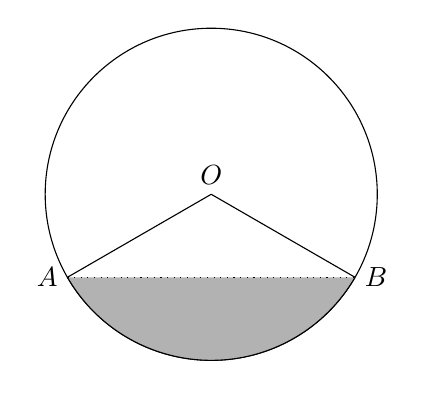
\begin{tikzpicture}
   \draw (0,0) node[above]{\(O\)} circle (60pt);
   \draw (-51.96152pt,-30pt) node[left]{\(A\)} -- (0,0);
   \draw (51.96152pt,-30pt) node[right]{\(B\)} -- (0,0);
   \filldraw[color=white!70!black,draw=black] (-51.96152pt,-30pt) arc (210:330:60pt);
   \draw[dotted](-51.96152pt,-30pt) -- (51.96152pt,-30pt);
  \end{tikzpicture}
 \]
 Given that \(\theta \) is sufficiently small for \(\theta^4\) and higher powers of \(\theta \) to be neglected, find the approximate area of the shaded region in terms of powers of \(\theta \).\hfill[5]
 \begin{answer}
  \begin{align*}
   \textrm{Area of Segment }AOB & = \textrm{Area of Sector }AOB -\textrm{Area of } \Delta AOB                                                                        \\
                                & = (4)\left(\frac{2\pi}{3}+\theta \right) - \frac{1}{2}\cdot{4}^2 \sin {\left(\frac{2\pi}{3}+\theta\right)}                         \\
                                & = \frac{8\pi}{3}+4\theta - 8\left(\sin{\frac{2\pi}{3}}\cos{\theta}+\cos{\frac{2\pi}{3}}\sin{\theta}\right)                         \\
                                & = \frac{8\pi}{3}+4\theta - 8\left({\frac{\sqrt{3}}{2}}\cos{\theta}-\frac{\sqrt{3}}{2}\sin{\theta}\right)                           \\
                                & = \frac{8\pi}{3}+4\theta - 4\sqrt{3}(\cos{\theta}-\sin{\theta})                                                                    \\
                                & = \frac{8\pi}{3}+4\theta - 4\sqrt{3}(\cos{\theta}-\sin{\theta})                                                                    \\
                                & = \frac{8\pi}{3}+4\theta - 4\sqrt{3}\left(1-\frac{\theta^2}{2!} + \cdots - \left(\theta-\frac{\theta^3}{3!} + \cdots\right)\right) \\
                                & = \frac{8\pi}{3}-4\sqrt{3}+(4+4\sqrt{3})\theta + 2\sqrt{3}\;\theta^2-\frac{2\sqrt{3}}{3}\theta^3+\cdots
  \end{align*}
 \end{answer}
 \1 It is given that \(y=\sqrt[3]{(1+x^2)(1+4x^2)}\). %Question 3

 \2 State the Maclaurin's expansion of \(y\) in ascending powers of \(x\) up to and including the \(x^4\) term.\hfill[4]
 \begin{answer}
  We will express \(y\) as a product of two Maclaurin expansions and collect the \(x^0\), \(x^2\) and \(x^4\) terms to simplify the expression.
  \begin{align*}
   y & =\sqrt[3]{(1+x^2)(1+4x^2)}                                                                                                                                                            \\
     & = {(1+x^2)}^{\frac{1}{3}}{(1+4x^2)}^{\frac{1}{3}}                                                                                                                                     \\
     & = \left(1+\frac{1}{3}x^2+\frac{\big(\frac{1}{3})\big(-\frac{2}{3})}{2!}x^4+\cdots\right)\left(1+\frac{1}{3}(4x^2)+\frac{\big(\frac{1}{3})\big(-\frac{2}{3})}{2!}(16x^4)+\cdots\right) \\
     & = \left(1+\frac{1}{3}x^2-\frac{1}{9}x^4+\cdots\right)\left(1+\frac{4}{3}x^2-\frac{16}{9}x^4+\cdots\right)                                                                             \\
     & = 1 + \frac{5}{3}x^2 - \frac{13}{9}x^4 +\cdots
  \end{align*}
 \end{answer}
 \2 Hence, show that \(\frac{91487}{90000}\) is an accurate estimate for \(\sqrt[3]{1.0504}\)  up to 4 d.p..\hfill[3]
 \begin{answer}
  We first evaluate \(\sqrt[3]{1.0504}\) up to 4 decimal places using our G.C., getting a result of 1.0165. To obtain the fraction above, we use the substitution \(x=0.1\) i.e. \(\sqrt[3]{(1+0.1^2){(1+4(0.1))}^2}=\sqrt[3]{1.0504}\). Since \(x\) is sufficiently small, we use the Maclaurin expansion in \textbf{(a)} to estimate \(\sqrt[3]{1.0504}\).
  \begin{align*}
   \sqrt[3]{1.0504} = \left.y\right|_{x=0.1} & \approx 1 + \frac{5}{3}{(0.1)}^2 - \frac{13}{9}{(0.1)}^4 \\
                                             & = \frac{91487}{90000}                                    \\
                                             & = 1.0165\dot{2}                                          \\
                                             & = 1.0165 \textrm{ (to 4 d.p.)}
  \end{align*}
 \end{answer}

 \1 Given that \(y=2^{\sin^{-1}{x}}\), where \(\sin^{-1}{x}\) denotes the principal value;
 \2 Show that:
 \begin{equation*}
  \dfrac{\mathrm{d}^2y}{\mathrm{d}x^2}=\dfrac{1}{y}{\left(\dfrac{\mathrm{d}y}{\mathrm{d}x}\right)}^2+\dfrac{x}{1-x^2}\cdot \dfrac{\mathrm{d}y}{\mathrm{d}x}.
 \end{equation*}\hfill[4]
 \begin{answer}
  By repeated Differentiation w.r.t. \(x\),
  \begin{align*}
   \frac{\mathrm{d}y}{\mathrm{d}x}     & =\frac{\mathrm{d}}{\mathrm{d}x}\mathrm{e}^{(\ln{2})(\sin^{-1}{x})}                                                                                                    \\
                                       & = \mathrm{e}^{(\ln{2})(\sin^{-1}{x})}\left(\frac{\ln{2}}{\sqrt{1-x^2}}\right)                                                                                         \\
                                       & = y\left(\frac{\ln{2}}{\sqrt{1-x^2}}\right)                                                                                                                           \\
   \frac{\mathrm{d}^2y}{\mathrm{d}x^2} & = \frac{\mathrm{d}y}{\mathrm{d}x}\left(\frac{\ln{2}}{\sqrt{1-x^2}}\right) + y(\ln{2})\left(-\frac{1}{2}\right){(1-x^2)}^{-\frac{3}{2}}(-2x)                           \\
                                       & = \frac{\mathrm{d}y}{\mathrm{d}x}\left(\frac{1}{y}\cdot\frac{\mathrm{d}y}{\mathrm{d}x}\right) + y\left(\frac{\ln{2}}{\sqrt{1-x^2}}\right)\left(\frac{x}{1-x^2}\right) \\
                                       & = \frac{1}{y}{\left(\frac{\mathrm{d}y}{\mathrm{d}x}\right)}^2+\frac{x}{1-x^2}\cdot \frac{\mathrm{d}y}{\mathrm{d}x} \textrm{ (shown)}
  \end{align*}
 \end{answer}
 \2 Hence, obtain the first three terms in the Maclaurin's series for \(y\).\hfill[3] %Question 4
 \begin{answer}
  The formula we want is \(\textrm{f}(x)=\textrm{f}(0)+x\textrm{f}^{\prime}(0)+\frac{x^2}{2!}\textrm{f}^{\prime \prime}(0)+\cdots+\frac{x^n}{n!}\textrm{f}^{(n)}(0)+\cdots \), which can be found in the MF26.
  \begin{align*}
   \left.y\right|_{x=0}                                   & =2^0=1                                                \\
   \left.\frac{\mathrm{d}y}{\mathrm{d}x}\right|_{x=0}     & =(1)\left(\frac{\ln{2}}{\sqrt{1-0^2}}\right) = \ln{2} \\
   \left.\frac{\mathrm{d}^2y}{\mathrm{d}x^2}\right|_{x=0} & =\frac{1}{1}{(\ln{2})}^2+0                            \\
                                                          & = {(\ln{2})}^2                                        \\
   \therefore y                                           & = 1 + x\ln{2} + \frac{x^2{(\ln{2})}^2}{2} + \cdots
  \end{align*}
 \end{answer}

 \1 The graph of \(y=\textrm{f}(x)\) is given by: % Question 5
 \begin{equation*}
  \textrm{f}(x) = \begin{cases}
   \mathrm{e}^{1/x^2}, & \textrm{for }  x\neq0 \\
   0                   & \textrm{for } x=0
  \end{cases}
 \end{equation*}
 \2 Show that \(\textrm{f}(x)\) is not equal to the Maclaurin Series of \(\mathrm{e}^{1/x^2}\).\hfill[3]
 \begin{answer}
  We will first find the Maclaurin expansion of \(\mathrm{e}^{1/x^2}\), which is in the form \(\mathrm{e}^{g(x)}\).
  \begin{align*}
   \mathrm{e}^{1/x^2}=1+\frac{1}{x^2}+\frac{1}{2x^4}+\cdots+\frac{1}{r!x^{2r}}+\cdots
  \end{align*}
  As \( x\rightarrow0 \) it is evident that the Maclaurin Series does not converge to 0, thus \(f(x)\) is not equal to its Maclaurin Series
 \end{answer}
 \2 Graph the function in \textbf{(a)}, labelling clearly the points at/around the origin.\hfill[3]
 \begin{answer}
  \vspace{3mm}
  \color{black}
  \begin{tikzpicture}
   \begin{axis}[
     axis lines = center,
     xlabel = $x$,
     ylabel = $y$,
     ymin=-1, ymax=20,
     legend pos=outer north east
    ]
    \addplot [
     domain=(-2:-0.5),
     samples=100,
     color=blue,
    ]
    {e^(1/(x^2))};
    \addplot [
     domain=(0.5:2),
     samples=100,
     color=blue,
    ]
    {e^(1/(x^2))};
    \addlegendentry{$\textrm{f}(x)$};
    \node[label={120:{$(0,0)$}},circle,fill,inner sep=2pt] at (axis cs:0,0) {};
   \end{axis}
  \end{tikzpicture}
 \end{answer}

 \1 Given that \(\tan{2x}=a_{0}+a_{1}x+a_{2}x^2+a_{3}x^3\cdots \), by using the fact that \(\sin{2x}=\cos{2x}\cdot \tan{2x}\), obtain the expansion of \(\tan{2x}\) in ascending powers of \(x\), up to and including the term in \(x^3\).\hfill[5] %Question 6
 \begin{answer}
  By expressing \(\sin{2x}\) and \(\cos{2x}\) in terms of their Maclaurin expansions, we can find each \(a_{j}\) for \(j=0,1,2,3\) by comparing coefficients on the LHS and RHS of the equation.
  \begin{align*}
   \sin{2x}                       & =\cos{2x}\cdot \tan{2x}                                                 \\
   2x-\frac{1}{3!}{(2x)}^3+\cdots & = (1-\frac{1}{2!}{(2x)}^2+\cdots)(a_{0}+a_{1}x+a_{2}x^2+a_{3}x^3\cdots) \\
   2x-\frac{4}{3}x^3+\cdots       & = a_{0}+a_{1}x+(a_{2}-2a_{0})x^2+(a_{3}-2a_{1})x^3+\cdots
  \end{align*}
  Comparing coefficients, we have \(a_{0}=0,\; \; a_{1}=2,\; \; a_{2}-2a_{0}=a_{2}=0\) \; and \( \; \;a_{3}-2a_{1}=a_{3}-4=-\frac{4}{3}\implies a_{3}=\frac{8}{3}\). Therefore, we have \(\tan{2x}=2x+\frac{8}{3}x^3+\cdots \).
 \end{answer}

 \1 It is given that \(\textrm{f}(x)=\dfrac{a-b}{(1-ax)(1-bx)}\), where \(a,b>0\). %Question 7

 \2 By expressing \(\textrm{f}(x)\) in terms of partial fractions and considering their Maclaurin expansions, show that:
 \begin{equation*}
  \sum_{r=0}^{\infty}(a^{r+1}-b^{r+1})x^{r}
 \end{equation*}\hfill[4]
 \begin{answer}
  \begin{align*}
   \frac{a-b}{(1-ax)(1-bx)} & \equiv \frac{A}{1-ax} + \frac{B}{1-bx} \textrm{ for some \(A,B\in \mathbb{R}\)} \\
   a-b                      & = A(1-bx) + B(1-ax)
  \end{align*}
  By first substituting \(x=\frac{1}{a}\) and then \(x=\frac{1}{b}\), we obtain \(A=a\) and \(B=-b\) respectively. We now use the expansion of \({(1+x)}^n\) which can be found in the MF26.
  \begin{align*}
   \textrm{f}(x) & =\frac{a-b}{(1-ax)(1-bx)}                                         \\
                 & = \frac{a}{1-ax} - \frac{b}{1-bx}                                 \\
                 & = a{(1-ax)}^{-1} - b{(1-bx)}^{-1}                                 \\
                 & = a(1+ax+a^2x^2+\cdots) - b(1+ax+a^2x^2+\cdots)                   \\
                 & = a\sum_{r=0}^{\infty}{a^r}{x^r} - b\sum_{r=0}^{\infty}{b^r}{x^r} \\
                 & = \sum_{r=0}^{\infty}(a^{r+1}x^r - b^{r+1}x^r)                    \\
                 & = \sum_{r=0}^{\infty}(a^{r+1}-b^{r+1})x^r
  \end{align*}
 \end{answer}

 \2 Hence or otherwise, prove that, if \(x^3\) and higher powers of \(x\) may be neglected, then \(\dfrac{2}{(1-5x)(1-3x)} \approx 2+16x+98x^2\).
 \hfill[2]
 \begin{answer}
  We will obtain the answer by setting \(a=5,b=3\).
  \begin{align*}
   \frac{2}{(1-5x)(1-3x)} & = \sum_{r=0}^{\infty}(5^{r+1}-3^{r+1})x^r  \\
                          & \approx \sum_{r=0}^{2}(5^{r+1}-3^{r+1})x^r \\
                          & = (5-3) + (5^2 - 3^2)x + (5^3 - 3^3)x^2    \\
                          & = 2 + 16x +98x^2 \textrm{ (shown)}
  \end{align*}
 \end{answer}

 \1 Find the Maclaurin's Series for \(\mathrm{e}^{ix}\) up to and including the coefficient of \(x^7\). \hfill[3] % Question 8
 \begin{answer}
  Using the standard series provided in MF26:
  \begin{align*}
   \mathrm{e}^{ix} = 1 + ix - \frac{1}{2!}x^2 - i\frac{1}{3!}x^3 + \frac{1}{4!}x^4 + i\frac{1}{5!}x^5 - \frac{1}{6!}x^6 - i\frac{1}{7!}x^7+ \cdots
  \end{align*}
 \end{answer}
 \2 Hence, prove that \(\mathrm{e}^{ix} = \cos x + i\sin x\). \hfill[3]
 \begin{answer}
  We notice that
  \begin{align*}
   \mathrm{e}^{ix} & = 1 + ix - \frac{1}{2!}x^2 - i\frac{1}{3!}x^3 + \frac{1}{4!}x^4 + i\frac{1}{5!}x^5 - \frac{1}{6!}x^6 - i\frac{1}{7!}x^7+ \cdots                            \\
                   & = \sum_{r=0}^{\infty} \frac{{(-1)}^r x^{2r}}{(2r)!} + i\sum_{r=0}^{\infty} \frac{{(-1)}^r x^{2r+1}}{(2r+1)!} = \cos x + i\sin x \quad\textrm{(shown)}\quad
  \end{align*}
 \end{answer}
\end{outline}

\end{document}
